\chapter{Entwickler}  % Kapitel % Steht dann über dem Text
\label{chapter:Entwickler}  % Steht als Text im Inhaltsverzeichnis
\index{Entwickler} % für das Stichwortverzeichnis

Als Entwickeler von CoderRed möchten wir uns gerne hier kurz vorstellen, wir stehen allen die weitere Fragen zu diesem Projekt haben natürlich gerne zur Verfügung. \\
\\
Allgemein besteht das Entwickelerteam von CodeRed aus zwei Studierenden der Staatlichen Techniker Schule Weilburg. Wir haben im Jahr 2004 die Ausbildung zum Staatlichen Techniker der Informationstechnik, Schwerpunkt Computersystem und Netzwerktechnik begonnen und Sommer 2005 dieses Projekt übernommen. Für uns stand bei der Übernahme der Aufgabe vorallem eines im Vordergrung, wir wollen unbedingt etwas machen was wir noch nicht beherschen und wir viel Lernen könnten. So war die Entwicklung eines Webbasierenden Trouble Ticket System eine nahe zu ideale Aufgabe, auch wenn wir erst nicht wussten wie wir diese Aufgabe lösen sollten.   
\pagebreak
\\
Backend Entwickeler \\
\textbf{Marco Benecke}
\\
\begin{figure}[h]
\begin{center}
   
\includegraphics[width=150pt]{../bilder/marcob.jpg}
   \caption{Entwickler -Marco Benecke}
   \label{Entwickler - Backend und Datenbank}
\end{center}
\end{figure}
\\
Marco Benecke \\
Bitzengarten 16 \\
35614 Asslar-Oberlemp \\
\\
\textbf{Konatkt} \\
\begin{itemize}
\item Mobil: 0175 - 74 10 565
\item E-Mail: benecke@gmail.com
\item JabberID: Risktaker@jabber.org 
\item Homepage: \href{http://www.bytes-delivery.de}{bytes-delivery.de}
\end{itemize}
\textbf{Werdegang} \\
\begin{itemize}
\item Realschulabschluss auf der Gesamtschule Asslar-Hermannstein
\item Ausbildung zum Energieelektroniker-Betriebstechnik bei der Buderus Guss GmbH in Wetzlar
\item 5./Technische Schule der Luftwaffe in Erndtebrück Staabsgebiet 6 – Netzbetreuer und Administrator
\item Weiterbildung zum Staatlich geprüften Techniker in Weilburg, Schwerpunkt: Computersystem und Netzwerktechnik	
\end{itemize}
\pagebreak
FrontEnd Entwickeler \\
\textbf{Jan Neuser}
\\
\begin{figure}[h]
\begin{center}
   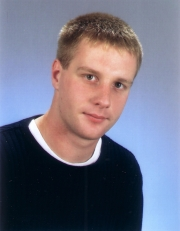
\includegraphics[width=150pt]{../bilder/jan.jpg}
   \caption{Entwickler -Jan Neuser}
   \label{Entwickler - Frontend und Datenbank}
\end{center}
\end{figure}
\\
Jan Neuser \\
Münchbornstr.4 \\
35753 Greifenstein Arborn \\
\\
\textbf{Konatkt} \\
\begin{itemize}
\item Mobil: 0177 - 60 39 783
\item E-Mail: jan@truematrix.de
\item JabberID: nean77@gmail.com 
\item Homepage: \href{http://www.truematrix.de}{truematrix.de}
\end{itemize}
\textbf{Werdegang} \\
\begin{itemize}
\item Realschulabschluss auf der Gesamtschule Driedorf
\item Ausbildung zum IT- Systemelektroniker in Sinn bei der Firma Dietermann \and Heuser GmbH  (Heute: Hees Bürowelt)
\item Stabskompanie Panzerbrigade 14, Stabsdienst - Truppenverwaltung
\item Weiterbildung zum Staatlich geprüften Techniker in Weilburg, Schwerpunkt: Computersystem und Netzwerktechnik	
\end{itemize}


